\documentclass[11pt]{article}
\usepackage{geometry}                
\geometry{letterpaper}                   

\usepackage{graphicx}
\usepackage{amssymb}
\usepackage{epstopdf}
\usepackage{hyperref}
%\usepackage{natbib}
\usepackage{amssymb, amsmath}
\DeclareGraphicsRule{.tif}{png}{.png}{`convert #1 `dirname #1`/`basename #1 .tif`.png}

\title{Agent-based computational approach modelling dynamics between civilians and organised groups}
%\author{Name 1, Name 2}
%\date{date} 

\begin{document}



\thispagestyle{empty}

\begin{center}
\includegraphics[width=5cm]{ETHlogo.eps}

\bigskip


\bigskip


\bigskip


\LARGE{ 	Lecture with Computer Exercises:\\ }
\LARGE{ Modelling and Simulating Social Systems with MATLAB\\}

\bigskip

\bigskip

\small{Project Report}\\

\bigskip

\bigskip

\bigskip

\bigskip


\begin{tabular}{|c|}
\hline
\\
\textbf{\LARGE{Agent-based computational approach }}\\
\textbf{\LARGE{modelling dynamics between civilians}}\\
\textbf{\LARGE{and organised groups}}\\
\\
\hline
\end{tabular}
\bigskip

\bigskip

\bigskip

\LARGE{Otto Schullian \& Stefano Weidmann}



\bigskip

\bigskip

\bigskip

\bigskip

\bigskip

\bigskip

\bigskip

\bigskip

Zurich\\
December 2014\\

\end{center}



\newpage

%%%%%%%%%%%%%%%%%%%%%%%%%%%%%%%%%%%%%%%%%%%%%%%%%

\newpage
\section*{Agreement for free-download}
\bigskip


\bigskip


\large We hereby agree to make our source code for this project freely available for download from the web pages of the SOMS chair. Furthermore, we assure that all source code is written by ourselves and is not violating any copyright restrictions.

\begin{center}

\bigskip


\bigskip


\begin{tabular}{@{}p{3.3cm}@{}p{6cm}@{}@{}p{6cm}@{}}
\begin{minipage}{3cm}

\end{minipage}
&
\begin{minipage}{6cm}
\vspace{2mm} \large Stefano Weidmann

 \vspace{\baselineskip}

\end{minipage}
&
\begin{minipage}{6cm}

\large Otto Schullian

\end{minipage}
\end{tabular}


\end{center}
\newpage

%%%%%%%%%%%%%%%%%%%%%%%%%%%%%%%%%%%%%%%



% IMPORTANT
% you MUST include the ETH declaration of originality here; it is available for download on the course website or at http://www.ethz.ch/faculty/exams/plagiarism/index_EN; it can be printed as pdf and should be filled out in handwriting


%%%%%%%%%% Table of content %%%%%%%%%%%%%%%%%

\tableofcontents

\newpage

%%%%%%%%%%%%%%%%%%%%%%%%%%%%%%%%%%%%%%%



\section{Abstract}
We propose a new agent-based model simulating civil violence in scenarios including civilian population, the government and multiple criminal organisations, for example a drug war. The gangs try to dominate the space by either exterminating opposing gangs or by winning over civilian population. The police want to counteract the recruitment, but also to suppress criminal activity. Both the government and the gangs can decide to help the civilians or to attack the gangs. The civilians may get more or less angry at the government and the gangs, which makes it more or less likely for them to join the gang, respectively.  We were mostly interested in the government-civilian relationship and especially how the help-attack ratio of the police affects the result of the simulation.
We found that the help-attack can have both a positive and negative impact on the result, depending on the initial parameters. The best result can be obtained, if the government employs a inversely proportional help-attack strategy compared to the help-attack ratio of the gang.
\section{Individual contributions}
Every group member contributed equally to the project.
\section{Introduction and Motivations}
Many countries in this world, even highly industrialised ones, such as Italy for example, are pestered with criminal gangs and the government can't seem to get a handle on it. Often several gangs struggle for supremacy, which results in bloody and fierce battles harming gang members as well as the civilian population. Criminal gangs may also approach civilians for gaining their confidence (one hand washes the other hand). Civilians may then tend to support them. 

The government's intentions are twofold: on the one hand they try to save and protect the civilians, on the other hand they try to suppress gang activity. One often excludes the other, which makes the task even more difficult. Therefore the dynamics of such a system should be examined and understood. More specifically, the important role the government-civilian relationship takes on and how they influence the dynamics and as well as the final equilibrium. We propose an agent-based simulation based on the work of Epstein \cite{epstein} and Bennett \cite{bennett} in such a way that the most interesting aspects of each paper is present, i.e. the risk calculation from \cite{epstein} and the civilian-to-gang conversion from \cite{bennett}. Additional features were added, such as helpful gestures from both the government and criminal gangs, in order to even better simulate the civilian-agent interactions. Also the influence of multiple gangs, in our case two opposing criminal organizations, was examined. The model may oversimplify the complexity of the problem but can easily be extended and even so yielded some interesting results. 

Whereas most papers, notably \cite{bennett}, and previous projects \cite{kouzoupis} are more concerned with the influence of efficiency and accuracy of the police on the outcome of the simulation, we were far more interested in the following questions and the long-term equilibria resulting from initial parameters. 
\begin{itemize}
\item Do such equilibria even exist, which are not either immediate death of the criminal gangs or complete take over? 
\item Which of the used parameters (attack probability, risk threshold, gang conversion threshold) has the biggest influence on the long-term outcome of the simulation?
\item How can the dependence of the outcome be related to the initial values (qualitatively)?
\item Which of the most influential parameters could be controlled by the government?
\end{itemize}

\section{Description of the Model}
We propose an agent based simulation featuring three different types of agents: civilians, policemen and any number of rivalling criminal gangs. The simulation is strongly based on \cite{epstein, bennett}. The `world' on which the simulation takes place is a rectangular grid. The initial positions of the agents (and the free positions) are random. During time propagation random agents have the possibility to move or to interact with other agents in their vicinity. 

Each civilian can be more or less angry at the police and the gangs. This anger will affect the decision of the civilian to join a gang. For example if the civilian is very angry at the police but not at all at one of the gangs, he will tend to join that gang. 

The gang's main aim is to dominate over the police and other gangs, i.e. to increase their size. This can be achieved by two approaches: one to kill the other gangs off, or to recruit new members among the civilians. Recruitment can be achieved by continuous helpful gestures towards civilians. This will decrease their anger at the gang and make it more likely for them to join. Attacking the other gang must be well considered by taking all possible risks into account, which is the inherent danger of a fight and the threat posed by nearby policemen. If the gang member still finds the risk low enough he will attack the other gang member. The outcome of the fight depends on the efficiency of both opponents. The loser  dies and is replaced by a new civilian. When an attack occurs there is a possibility of collateral damage among the civilian populationtrade-off, which in our simulation will lead to an increase in anger, which on the other hand will make it less likely for the civilian to join the gang.

The police's main aim is to protect civilians and to suppress criminal activity. These are two courses of action, that often do not coincide. This trade-off is simulated by a probability to attack or to help. Most of the police agents' actions are very similar to the gang members', with a few exceptions. Since they cannot recruit from the civilian population they cannot die (otherwise they would certainly die out in the simulation). Also they will not be attacked by the criminal gangs, who want to operate in the dark. Similarly to gang agents, a policeman can attack, after a careful risk assessment, but if he does so, collateral damage can be the consequence, increasing the civilian's anger. Helping on the other hand will decrease their anger. 

  
\section{Implementation}
The world or space modelled consists of a rectangular grid with edge boundaries. Toroidal boundaries could be easily implemented, however, we think that edges represent the real world more realistically.

Agents may interact with their surroundings by either agent-agent interactions or by movement to a free neighbouring cell. The interaction range is a Moore neighbourhood and the vision range can be specified for each type individually, but is generally set to 1, i.e. a Moore neighbourhood of size 9. The different types of agents are distinguished as follows.

\subsection{Civilians}

The civilian is attributed an Anger/Fear value $A \in [0,1]$ each for the police and every criminal gang. This values will determine whether a civilian joins a gang, more specifically if for a randomly chosen civilian agent
\begin{equation}
A_{\text{police}}-A_{\text{gang}_i}>T_{\text{conversion}},\label{angerdiff}
\end{equation}
where $T_{\text{conversion}} \in [0,1]$ is the conversion threshold specified globally, the conversion takes place, and the algorithm will replace the civilian with  
a new gang member with the same coordinates. Every new civilian that enters the simulation is assigned an initial anger value for the police and the gangs.

\subsection{Police}
The police agents are attributed an efficiency value $\epsilon\in [0,1]$ and an accuracy value $\alpha\in [0,1]$. These values are distributed among the police agents according to a Gaussian distribution with initially specified mean $\epsilon_0,\alpha_0$ and standard deviation $\sigma_\epsilon=0.25$, $\sigma_\alpha=0.25$. These will determine the outcome of a fight and the amount of collateral damage. Risk aversion $\rho\in [0,1]$ and attack threshold $T_{\text{attack}}$ determine whether an attack is carried out. Furthermore, a probability for attack $P_{\text{police}}$ is set globally, which determines whether a police agent considers attacking gang members or helping civilians. In addition, a change parameter $\gamma\in [0,1]$ is chosen globally, which will affect the anger of the civilian according to equations (\ref{angeradjust1}),(\ref{angeradjust2}) in the case of either collateral damage or helpful gesture. Police agents never die.
\subsection{Gangs}
The number of gangs can be chosen freely at the beginning of the simulation. The specified parameters for the gang members are the same as for the police agents, i.e. the efficiency (with mean $\epsilon_{0,\text{gang}}$), the accuracy (with mean $\alpha_{0,\text{gang}}$), the attack probability $P_{\text{gang}}$, the risk aversion $\rho_{\text{gang}}$, the attack threshold $T_{\text{attack,gang}}$ and the change parameter $\gamma_{\text{gang}}$. They can be interpreted similarly, but are varied separately from the police but not for different gangs. 
\subsection{Algorithm}
Initially, two matrices are generated. One representing the space (called \textit{gridpos}) and the other carrying information about all the agents in the simulation (called \textit{agents}). \textit{gridpos} has the form of a $n\times n$-matrix, each element pointing to a row in the \textit{agents} matrix. Each row in \textit{agents}  represents an agent with all their properties, including the position on \textit{gridpos}. After this initialization a loop simulates the time propagation. The loop consists of a movement phase and a agent-agent interaction. In the movement phase a random agent is assigned a new random free position. Subsequently, in the agent-agent interaction phase, a random agent is selected. The type of the agent is retrieved and depending on the type one of the following functions are executed
\begin{itemize}
\item \textit{civilian}: For each gang equation (\ref{angerdiff}) is calculated. If it is satisfied for any gang, the civilian will be replaced by a new gang member. If it is satisfied for more than one gang a random gang is chosen. 
\item \textit{police}: By means of the attack probability $P_{\text{police}}$ it is decided whether the police agent considers an attack or helping a civilian agent. If the police agent decides to help, a random civilian in his vision is selected, whose anger value $A_{\text{police}}$ is reduced by a fraction $\gamma_{\text{police}}$  according to equation
\begin{equation}
A_{\text{police,final}}=A_{\text{police,initial}}\cdot (1-\gamma_{\text{police}}).\label{angeradjust1}
\end{equation}
If the police agent decides to attack the risk for an attack is calculated. The net risk to attack a member of gang $i$ is given by
\begin{equation}
\nu_{\text{gang,i}}=\rho\cdot \left( 1-\exp\left(-k_\text{successful}\frac{N_{\text{gang,i}}}{N_\text{police}}\right)\right),\label{netriskpolice}
\end{equation}
where $\nu_{\text{gang,i}}$ is the net risk to attack gang $i$, $N$ the number of agents of the type specified in the index seen by the police agent. The second factor in equation (\ref{netriskpolice}) calculates the success of the attack. $k_\text{successful}$ is set such that if there is an equal number of police and gang, the success is 0.5. Having calculated a net risk for all gangs in the vision, the algorithm determines the minimum net risk. In the case of multiple gangs having the same minimum net risk one of these gangs is chosen randomly. If the minimum net risk is below $T_{ \text{attack}}$, the attack is carried out by selecting one random agent of the considered gang in the vision of the police agent. The relative efficiency, given by
\begin{equation}
\frac{\epsilon_{\text{police}}}{\epsilon_{\text{police}}+\epsilon_{\text{gang}}}
\end{equation}
gives the probability for killing the gang member. If the gang member is killed it is replaced by a civilian in the same position on the grid. If the attack fails nothing happens. The collateral damage among the civilians is considered next for both the attacking police agent and the target gang member. The civilians in the vision of the respective agent are retrieved and with the probability of $1-\alpha$, the anger of the civilian agent is increased according to 
\begin{equation}
A_{\text{final}}=A_{\text{initial}}+(1-A_{\text{initial}})\cdot \gamma.\label{angeradjust2}
\end{equation}
\item \textit{gang member}: The execution of the gang member function is very similar to the police function. One difference is, that the gang members will not attack the police agents. Therefore no net risk against the police is calculated. The net risk is also calculated differently taking into account police agents in the neighbourhood
\begin{eqnarray}
\nu_{\text{gang,i}}=\rho\cdot\frac{1}{2}\cdot \left\{\left( 1-\exp\left(-k_\text{successful}\frac{N_{\text{gang,i}}}{N_\text{own gang}}\right)\right)+\right.\\
 \left.\left( 1-\exp\left(-k_\text{arrest}\frac{N_{\text{police}}}{N_\text{own gang}}\right)\right)\right\},\label{netriskgang}
\end{eqnarray}
where $N_{\text{own gang}}$ denotes the number of gang agents in the vicinity of the same gang. The last term in the expression (\ref{netriskgang}) denotes the probability of getting arrested by police agents and $k_\text{arrest}$ is chosen such that the arrest probability for an equal number of police agents and own gang members is 0.9, similar to $k_\text{successful}$. The execution of the attack is the same with the only exception that the attacker can also die in the fight. In that case the attacker is replaced by a civilian agent. The collateral damage and the helpful gestures are both considered in the same way. 
 \end{itemize}



\section{Simulation Results and Discussion}
\subsection{General}
The simulations performed in this project were restricted to two rivalling gangs. The grid size was $30 \times 30$ cells and the number of time steps varied from 20000 to 100000. The initial agent ratios are given in table \ref{pop}.
\begin{table}[h!]
\centering
\begin{tabular}{lc}
\hline
agent type & density ratio\\
\hline
police & 0.1\\
civilians & 0.5\\
gang 1 & 0.15\\
gang 2 & 0.15\\
empty spaces & 0.1
\end{tabular}
\caption{Relative initial densities used in all our simulations.}\label{pop}
\end{table}
 Examples for the grid and the general output of the simulation can be found in \cite{epstein, bennett}. Since we were only interested in the outcome in terms of civilian population we only investigated those. 

\subsection{Sensitivity Analysis}\label{sensitivityanalysis}
A sensitivity analysis determines the amount of uncertainty influence of a model from the different input parameters.$^{\text{\cite{saltelli}}}$ An elaborate discussion on sensitivity analysis can be found in \cite{saltelli}. Variance based models have a long history and due to the properties of our model, where probabilities were used in many situations, we found that this approach would be the most rewarding. The model can mathematically be described by
\begin{equation}
Y=f(X_1,\ldots, X_n),
\end{equation}
where $Y$ is the result and $X_1,\ldots,X_n$ represent the $n$ input parameters. A variance based first order effect can be calculated as
\begin{equation}
V_{X_i}(E_{X_{\sim i}}(Y|X_i)),
\end{equation}
where $X_{\sim i}$ denotes the matrix of all factors but $X_i$. The expectation value is calculated for all possible values of $X_{\sim i}$, while keeping $X_i$ fixed. The associated sensitivity measure is then given by
\begin{equation}
S_i=\frac{V_{X_i}(E_{X_{\sim i}}(Y|X_i))}{V(Y)},\label{sensitivity}
\end{equation}
where $V(Y)=V_{X_i}(E_{X_{\sim i}}(Y|X_i))+E_{X_i}(V_{X_{\sim i}}(Y|X_i))$. $S_i$ denotes the first order (additive) effect of the initial parameters.$^{\text{\cite{saltelli}}}$

The simulations were performed at least once for every set of parameters, varying almost all the parameters from a minimal value to a maximum value (only two values), leading to at least $2^{12}=4096$ simulation results. The parameters can be seen in table \ref{varianceparameters}.

\begin{table}
\centering
\begin{tabular}{llc}
\hline
parameter && value \\
\hline
attack threshold  &$T_{\text{attack}}$ &0.1 - 0.6\\
risk aversion& $\rho$ &0.1\\
threshold for gang conversion \qquad & $T_{\text{conversion}}$ &0 - 0.6\\
attack probability police&  $P_{\text{police}}$ &0.1 - 0.9\\
attack probability gang&  $P_{\text{gang}}$ &0.1 - 0.9\\
change police& $\gamma_{\text{police}}$ &0.1 - 0.6\\
change gang &$\gamma_{\text{gang}}$& 0.1 - 0.6\\
mean accuracy police &$\alpha_{0,\text{police}}$ &0.1 - 0.9\\
mean accuracy gang &$\alpha_{0,\text{gang}}$ &0.1 - 0.9\\
mean efficiency police& $\epsilon_{0,\text{police}}$ &0.1 - 0.9\\
mean efficiency gang &$\epsilon_{0,\text{gang}}$ &0.1 - 0.9\\
initial anger police &$A_{\text{police,initial}}$ &0.1 - 0.5\\
initial anger gang &$A_{\text{gang,initial}}$ &0.1, 0.5\\
no. of time steps && 20000
\end{tabular}
\caption{Parameter values for the data aquisition for the sensitvity analysis. All possible combinations for the given parameters were used at least once.}\label{varianceparameters}
\end{table}

The sensitivity, in accordance with equation (\ref{sensitivity}), for the equilibrium number of civilians is displayed in fig. \ref{varianceequilibrium} The expectation values were calculated in two different ways. Once by taking the mean over the last data points (red bars in fig. \ref{varianceequilibrium}) and the second by fitting the simulation to two exponential decays, given by the equation
\begin{equation}
N_{\text{civ}}(t)=a\cdot e^{-bt}-c\cdot e^{-dt} +f,\label{fit}
\end{equation}
where $a,b,c,d$ and $f$ are fitting parameters $\ge 0$ and $t$ the time step. Since both exponentials will decay to $0$ after a certain time, the remaining equilibrium value is given by $f$. The second variance sensitivity analysis was performed on this factor $f$ (blue bars in fig. \ref{varianceequilibrium}). The fit of course is a gross oversimplification, but fits quite nicely in almost all cases. Whether the estimate for the future behaviour of the result with the fit is valid, remains unclear and should be tested in future simulations. However, so far no massive divergence between the evaluation using the fit data or the mean data was found.

A simple qualitative conclusion can immediately be drawn from the results shown in fig. \ref{varianceequilibrium}: the highest influence on the outcome of the simulation comes from the conversion threshold. This can easily be explained by the fact, that the lower the threshold is, the faster civilians will join the criminal gangs regardless of the response and behaviour of the police agents or criminal gangs. Next in line are the attack probability of the gang, the mean accuracy of the police and the mean efficiency of the police. Since they will determine the amount of gang agents dying in the process, which in turn are replaced by a new civilian agent, they will influence the outcome greatly. Contrary to our expectation, however, the attack probability of the police does not seem to have a major influence (or even a minor for that matter) on the outcome of the simulation. This seems very surprising at first, but in the end there will be a trade-off. The more the police attacks, the more gang members will die from police-gang member fights, which will increase the number of civilians, but due to collateral damage, make it more likely for them to join the gangs. On the other hand if the police does not attack as often, less gang members will die in fights with the police, but also less civilians will be recruited.
 
\begin{figure}[h!]
	\centering
	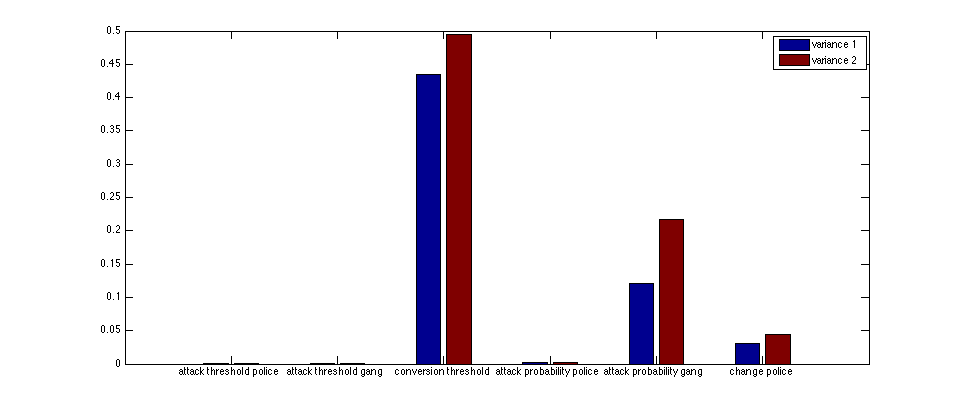
\includegraphics[width=\textwidth]{varianceeq1.png}
	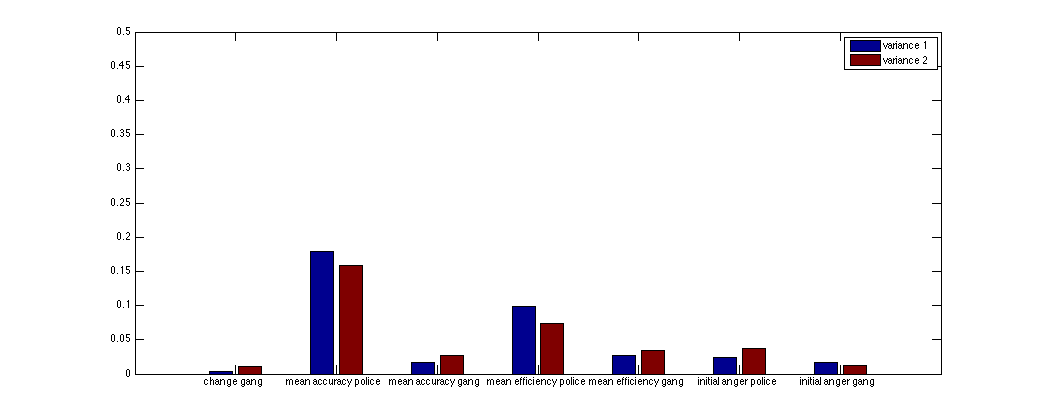
\includegraphics[width=\textwidth]{varianceeq2.png}
	\caption{The variance for the input variables calculated according to equation (\ref{sensitivity}). Two methods were used to calculate the expectation value, once using the mean of the last 2000 data points (red bars), and once fitting the output to a double exponential decay given in equation (\ref{fit}) (blue bars). Both methods however yield similar results.}\label{varianceequilibrium}
\end{figure}

\newpage
\subsection{Additional Characterisation}
In order to characterise the simulation more rigorously, simulations were carried out for a longer period, keeping all parameter at an average value except for one. Only the parameters with the highest variances were examined more closely. For each set of initial parameters, ten simulations were performed and the mean and standard deviations were calculated. Unless otherwise stated, the simulation parameters can be seen in table \ref{parameters}.
\begin{table}
\centering
\begin{tabular}{lll}
\hline
parameter && value \\
\hline
attack threshold police  &$T_{\text{attack,police}}$ &0.35\\
attack threshold gang& $T_{\text{attack,gang}}$& 0.35\\
risk aversion police& $\rho_{\text{police}}$ &0.35\\
risk aversion gang& $\rho_{\text{gang}}$ &0.35\\
threshold for gang conversion \qquad & $T_{\text{conversion}}$ &0.1\\
attack probability police&  $P_{\text{police}}$ &0.5\\
attack probability gang&  $P_{\text{gang}}$ &0.5\\
change police& $\gamma_{\text{police}}$ &0.35\\
change gang &$\gamma_{\text{gang}}$& 0.35\\
mean accuracy police &$\alpha_{0,\text{police}}$ &0.5\\
mean accuracy gang &$\alpha_{0,\text{gang}}$ &0.5\\
mean efficiency police& $\epsilon_{0,\text{police}}$ &0.5\\
mean efficiency gang &$\epsilon_{0,\text{gang}}$ &0.5\\
initial anger police &$A_{\text{police,initial}}$ &0.3\\
initial anger gang &$A_{\text{gang,initial}}$ &0.3\\
no. of time steps && 100000
\end{tabular}
\caption{General parameters for the more accurate analysis of the simulation. Except for the examined parameter the following results were obtained using these initial values.}\label{parameters}
\end{table}

\subsubsection{Threshold for Gang Conversion}
In this run the threshold for gang conversion was incremented stepwise by 0.2 from -0.4 to 0.8. According to the sensitivity analysis this threshold has the highest influence on the outcome of the simulation, which turned out to be true, within a certain range of the parameter values. The simulation results (averaged over 10 runs) are displayed in fig. \ref{gangconv}. 
\begin{figure}[h!]
	\centering
	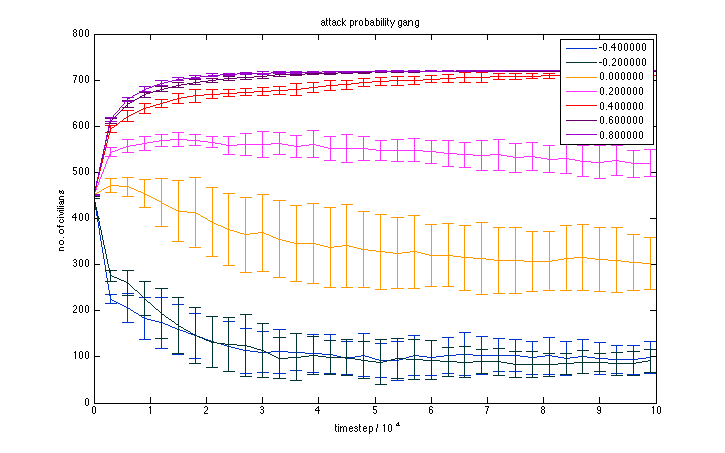
\includegraphics[width=11cm]{gangconv.png}
	\caption{Simulation results for different parameters of the gang conversion threshold $T_{\text{conversion}}$. }\label{gangconv}
\end{figure}
\newpage

As expected, the higher the threshold, the less likely is the recruitment, increasing the number of civilians. Looking more closely at the the final equilibrium values, one notices an almost linear dependence on the threshold over a range from -0.2 to 0.4, which is quite astonishing considering the highly randomised methods used in the algorithm. However, how this result is of practical use, is not too clear, since the conversion threshold is not a parameter that can be easily adjusted by the agents, but is rather a societal attitude, which is probably linked in some way to other initial parameters such as initial anger. 
\begin{figure}[h!]
	\centering
	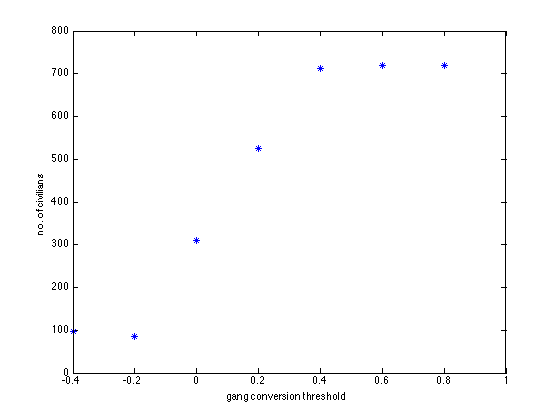
\includegraphics[width=11cm]{gangconv2.png}
	\caption{Simulation results for different parameters of the gang conversion threshold $T_{\text{conversion}}$. }\label{gangconv}
\end{figure}
\newpage
\subsubsection{Accuracy and Efficiency of the Police}
The influence of these parameters has already been extensively studied in \cite{bennett, kouzoupis} and will therefore not be repeated here. It will just be mentioned for the sake of completeness, that they the impact one would expect, i.e. high efficiency and high accuracy lead to a high number of civilians, and low values for the two parameters lead to low numbers of civilians.


\subsubsection{Attack Probabilities}
Investigating the influence of the attack probabilities of the police and the gangs was one of the major interests of this work.


The attack probability has been varied from 0.1 to 0.9 in increments of 0.2. The different parameter results have little overlap, as can bee seen in figure \ref{attackprobgang}.
The attack probability of the gangs apparently has a major impact on the outcome of the simulations. A higher attack probability produces a higher number of civilian agents at the end of a simulation. The increased number of gang member deaths, in addition to the increased anger due to collateral damage, lead to the higher number of civilians. The sensitivity analysis reflects this fact, ranking the attack probability for the gangs as one of the most important factors. 

\begin{figure}[h!]
	\centering
	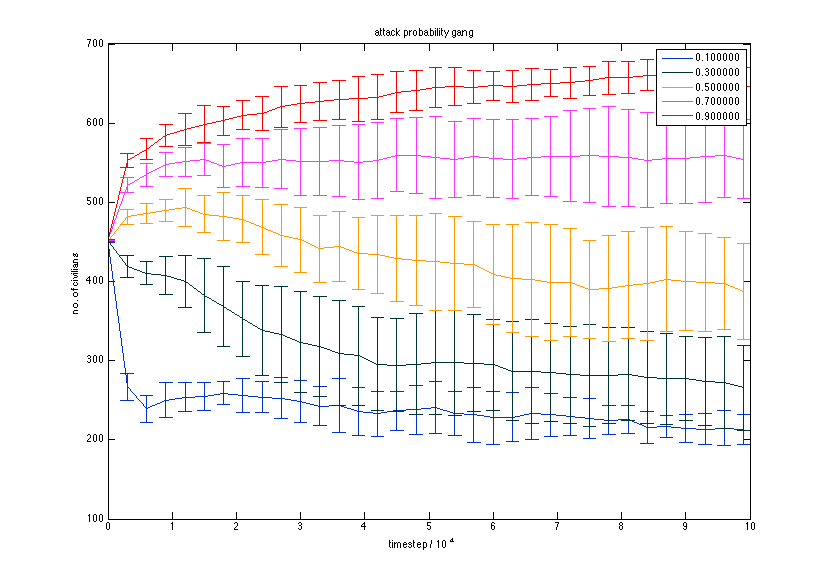
\includegraphics[width=9cm]{attackprobgang.png}
   \caption{Simulation results for different parameters of the attack probability of the gangs $P_{\text{gang}}$. }\label{attackprobgang}
\end{figure}


\begin{figure}[h!]
	\centering
	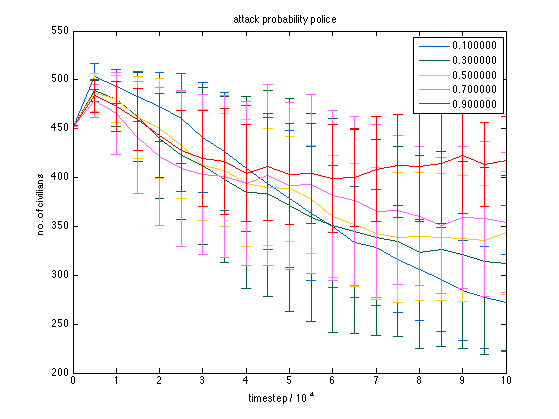
\includegraphics[width=9cm]{attackprobpolice.png}
   \caption{Simulation results for different parameters of the attack probability of the police $P_{\text{police}}$. }\label{attackprobpolice}
\end{figure}
The situation for the attack probability of the police however, is more interesting. 
Although according to the sensitivity analysis, it has a rather small effect, figure \ref{attackprobpolice} exhibits a remarkable pattern, not seen previously. The most pacifist behaviour of the police ($P_{\text{police}} = 0.1$) excels at the beginning of a simulation, but is surpassed by more aggressive strategies at some point during the simulation, leading to an inverting of the initially expected result.
This unexpected fact is further investigated comparing various combinations of the two attack probabilities (see fig. \ref{attackprob}).
As one can see again, the attack probability of the police is much less important than the attack probability of the gangs.
However, for a fixed gang attack probability, the minimum of the number of civilians seems to be dependent on the ratio of the two probabilities. Therefore, there seems to be a inverse correlation of the two probabilities for the maximum. A high attack probability for the gang leads to a maximum for a low probability for the police and vice versa. This could be caused by the fact, that a high collateral damage from the gangs, due to an increased number of fights, already leads to a high anger at the gangs. If the anger at the police would increase as well, the recruitment would be facilitated. A similar argument can be used for the converse scenario. If the anger at the gang is already low, a high anger at the police won't do as much damage to the outcome as attacking them as much as possible.
\begin{figure}[h!]
	\centering
	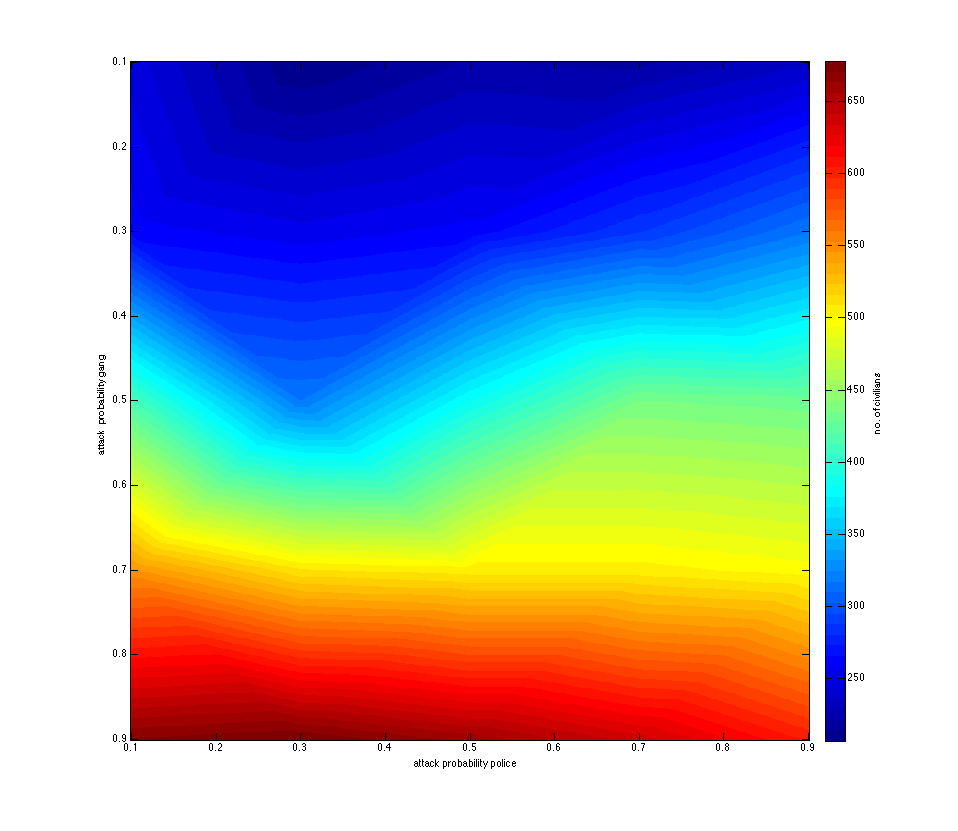
\includegraphics[width=9cm]{attackprob.png}
   \caption{The outcome of a simulation as function of the two attack probabilities}\label{attackprob}
\end{figure}
\newpage
\section{Summary and Outlook}
The simulation succeeds in simulating plausible results, based on this simple model. Results that were initially expected could be reproduced, which is fundamental for the reliable interpretation of the less obvious relations. All the simulations performed suggested that the system converges towards an equilibrium. Even for very long simulations no oscillatory effects were noticed. The sensitivity analysis performed in section \ref{sensitivityanalysis} clearly shows that the most influential parameter is the conversion threshold. Unfortunately this is a parameter, which is very hard to influence by the government, because it is more of a societal attitude and almost certainly linked to other parameters. Leaving that aside, the next most influential parameters, that can be changed by the government is the accuracy and efficiency of the police agents. Better training of the police agents will affect the outcome of such a scenario by a high percentage. This aspect however has already been thoroughly tested in previous work \cite{bennett,kouzoupis}. 

The parameter, that was of most interest in this work is the attack probability of the police, since it will determine the relationship between civilians and the government. According to the sensitivity analysis, the influence of that parameter is almost nonexistent. Analysing this parameter more thoroughly showed, that its influence is strongly related to the overall initial parameters, i.e. that in one case it can have a harmful influence, in others the influence can be helpful. We investigated the dependence on the attack probability of the gangs - which probably is one of the easiest parameters to monitor by the government - and found that the best response should be inversely proportional to the attack probability, i.e. the aggressiveness. If a gang is very aggressive, the government should, according to our model, be more supportive of the civilian population, this way only the anger against the gangs will increase. If the gangs on the other hand pursue the supportive strategy, the government should try to work against them more aggressively. 

As stated several times, some of the concepts used in this work oversimplify the situation and a lot of parameters were not considered. Future work should definitely include the implementation of the fear factor (as done in \cite{bennett}), which opposes the anger. Also the influence of parameter changes during the simulation should be examined (continuous or depending on the state of the simulation), since they would correspond to a strategy change.

\section{References}

\section{Appendix}
\begin{thebibliography}{sotief}
\bibitem{epstein} J. M. Epstein, \textit{PNAS}, \textbf{2002}, \textit{99 (3)}, 7243.
\bibitem{bennett} S. Bennett, \textit{JASSS}, \textbf{2008}, \textit{11(4)}, 7.  
\bibitem{saltelli} A. Saltelli, P. Annoni, I. Azzini, F. Campolongo, M. Ratto, S. Tarantola, \textit{COMPUT PHYS COMMUN}, \textbf{2010}, \textit{181}, 259.
\bibitem{kouzoupis} D. Kouzoupis, M. Rozou, M. Tsopelas, ``Governments, Civilians, and the Evolution of Insurgency: Modelling the Early Dynamics of Insurgencies'', ETH Zürich, \textbf{2011}.
\end{thebibliography}

\end{document}  



 
